% !TEX root = ../../../main.tex
% 来源：中学数学实验教材·第一册（代数）
% 章节：多项式的四则运算 / 一元多项式的除法
% 原始文件：4.tex，行 1780-1800
% 类型：tikz
% ---
         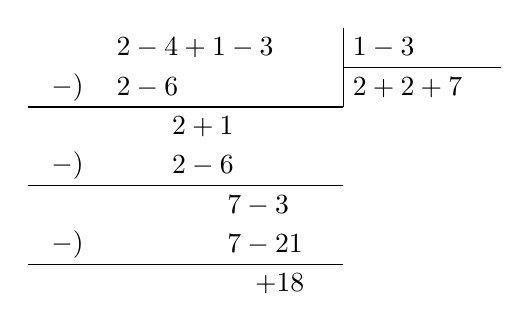
\begin{tikzpicture}
            \node at (0,.5) [right]{$2-4+1-3$};   
            \node at (0,0) [right]{$2-6$}; 
            \node at (0,-.5) [right]{\qquad $2+1$}; 
            \node at (0,-1) [right]{\qquad $2-6$}; 
            \node at (0,-1.5) [right]{\qquad \qquad $7-3$}; 
            \node at (0,-2) [right]{\qquad\qquad $7-21$}; 
           \node at (0,-2.5)[right]{\quad\qquad\qquad $+18$};
           
           \foreach \x in {-.25,-1.25,-2.25}
           {
               \draw (-1, \x)--(3,\x);
               \node at (-.5, \x+.25){$-)$};
           }
           
           \draw (3,.75)--(3,-.25);
           \draw (3,.25)--(5,.25);
           \node at (3,.5)[right]{$1-3$};
           \node at (3,0) [right]{$2+2+7$};
           
           \end{tikzpicture}
